% !TeX root = ../thuthesis-example.tex

\chapter{总体设计和系统概述}

% \section{发动机和油门控制器}

% 为 F-14B 提供动力的两台 F110-GE-400 带加力燃烧室涡轮风扇发动机由 AFTC(增推扇叶温度控制装置)进行控制。AFTC 类似于较新发动机中所使用的早期版 FADEC(全权数字发动机控制)。

% AFTC 控制发动机本身以及发动机排气的喷口的开闭。 除此之外,AICS(进气控制系统)通过控制进入发动机的气流来为发动机进口提供均匀的亚音速气流。AICS 是通过可调进气道——更准确地说,是通过进气道中的可调斜板来完成对气流的控制的。

% 这些控制都是通过 AFTC 和 AICS 使用合适的传感器输入,然后 AFTC 和 AICS 根据制度(注:调定程序)来控制发动机运行来实现的。

% 此外,两台发动机还将分别驱动的供油系统、液压系统和发电机,以此来增加余度。

% 在 AFTC 发生故障的情况下,MEC(主发动机控制)可以对发动机进行控制以提供备份机械控制。正常模式——AFTC——将其称为发动机的主要模式(PRI),而备份 MEC 称为次要(SEC)模式。如果 AFTC 中发生故障,那么次要模式或主要模式将被自动选用,但也可以手动选择次要或主要模式。值得一提的是,在次要模式下,除了加力燃烧被禁用外,喷口还将完全闭合并被禁用,两者都被禁用将导致发动机性能下降。

% \subsection{油门控制器}
% \begin{figure}[htb]
% 	\centering
% 	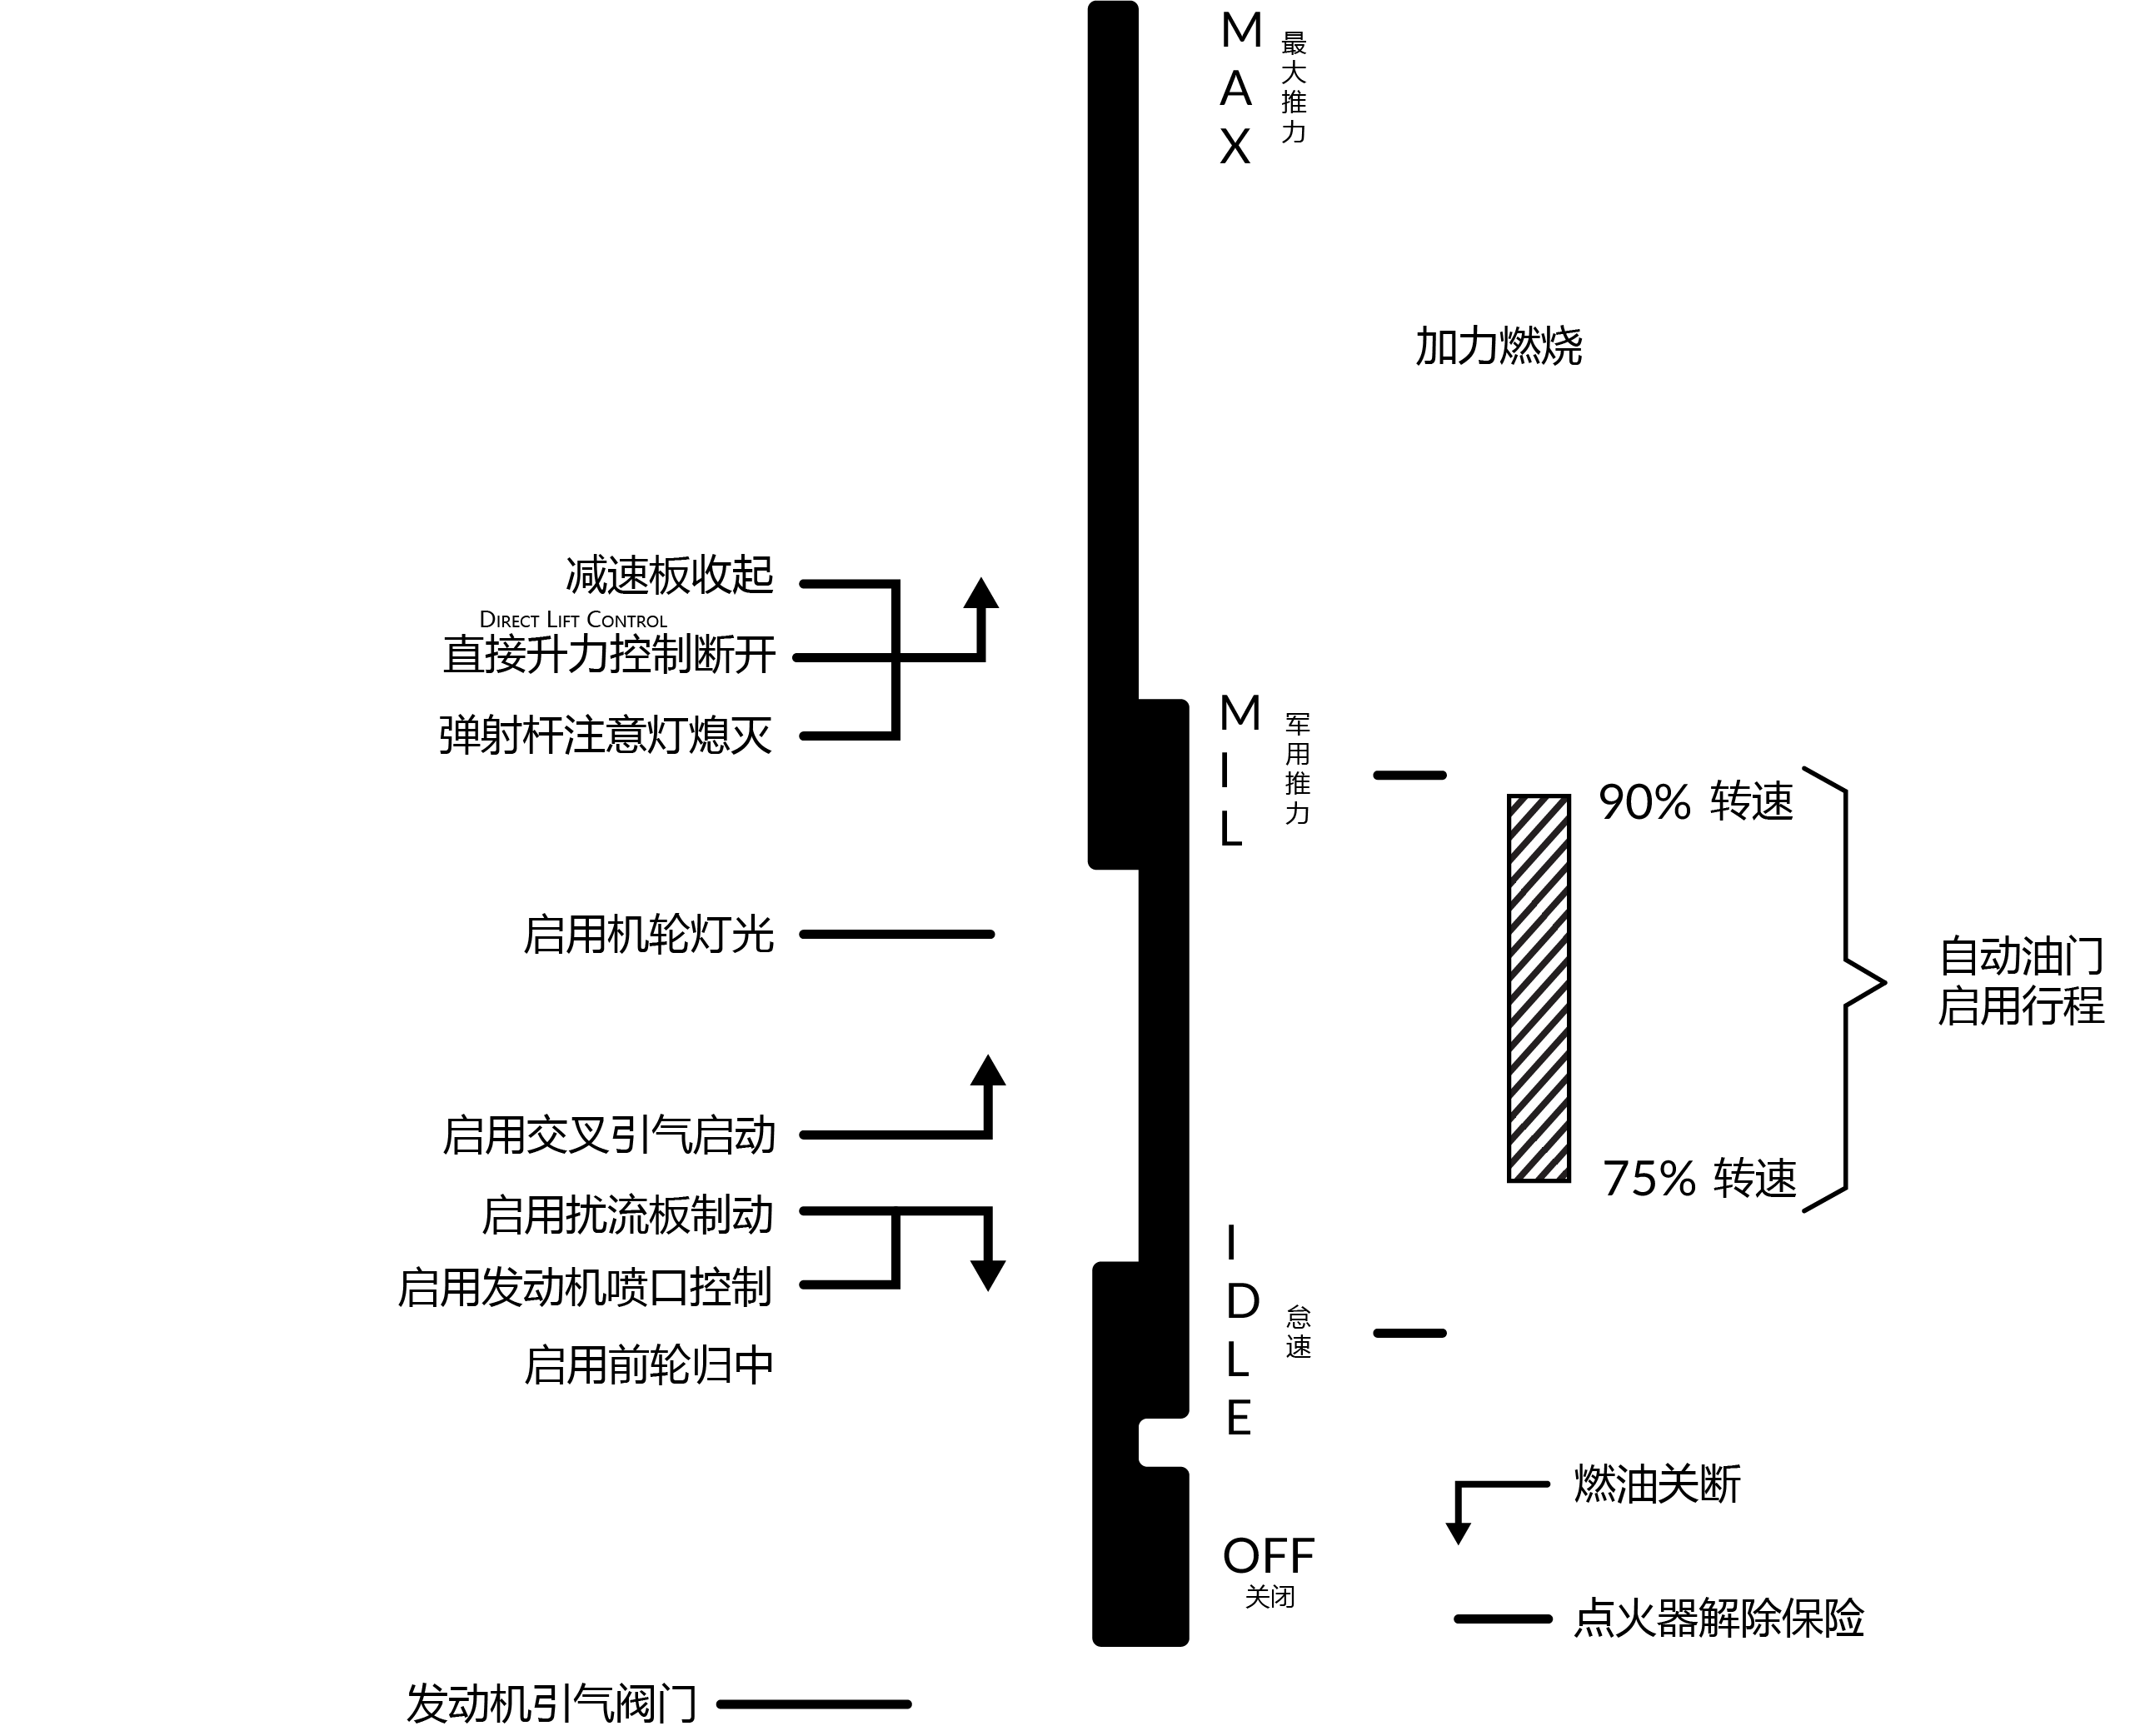
\includegraphics[width=0.6\textwidth]{throttles-schem1.png}
% \end{figure}

% F-14 的油门行程中含有数个限位机构以防止发动机意外启动或关闭发动机,或意外启用加力燃烧室。此外,如上图所示,油门还用来控制数个根据油门位置运作的不同的系统。这些系统中,其中最重要的是就是发动机燃油关断和点火系统。

% 油门有三种操作模式:

% MAN(手动模式)为机械操作模式,在手动模式下,油门通过机械传动机构直接连接到发动机来对其进行控制。手动模式被设计为备用模式,并且由于机械控制的特性,这种模式下对发动机的控制并不准确。

% BOOST(助力)模式,助力模式是油门的正常操作模式,在这个模式下,油门通过电力控制作动器来移动与机械传动机构相同的发动机控制器,但与手动模式不同的是,助力模式对发动机控制更加准确并且控制油门所需要的力更小。

% 第三种模式是进近推力补偿模式或称为自动油门模式,在自动油门模式下,自动油门控制系统允许使用自动油门控制来在进近中保持最佳迎角。

% 油门模式的控制开关位于主油门一旁的进气道斜板/油门控制面板中,控制开关可用来选择全部三种油门模式。使用 AUTO 模式时,开关将由螺线管固定在 AUTO 档位,如果不满足自动控制的条件,那么开关将恢复至助力模式。

% 如需选择自动油门模式,必须将油门置于处于75\%到90\% RPM 之间、起落架手柄位于放下档位以及机轮不负重。如果再不满足前述条件,那么可以用力移动油门来手动超控或按下左油门握把中的 CAGE/SEAM 按钮,按下后螺线管将释放开关并恢复至助力模式。

% 此外,飞行员还可以在进气道斜板 / 油门控制面板中设置自动油门系统的增益。增益设置分别为 HOT、NORM 和 COLD ,HOT 档位增加一般油门计算机增益(和有效推力),COLD 档位减小一般油门计算机增益。控制开关设置对应外部气温的“冷”和“热”,但飞行员应根据实际油门控制进行设置。

% RATS 或称为航降减推系统,航降减推系统将在触舰后限制发动机推力至适合舰上环境的水平。主起落架任意一侧机轮负重都将启用航降减推系统,并且可以通过推动油门选择加力燃烧来禁用 RATS。

% 最后,F110-GE-400 发动机上装备了不对称推力限制器(ASYM LIMITER),如果只有一侧发动机启用加力燃烧,那么不对称推力限制器将限制加力燃烧在最小加力推力直到另一侧发动机也启用加力燃烧来防止使用不对称加力燃烧。

% \subsection{发动机和油门控制开关以及指示器}
% \begin{figure}[htb]
% 	\centering
% 	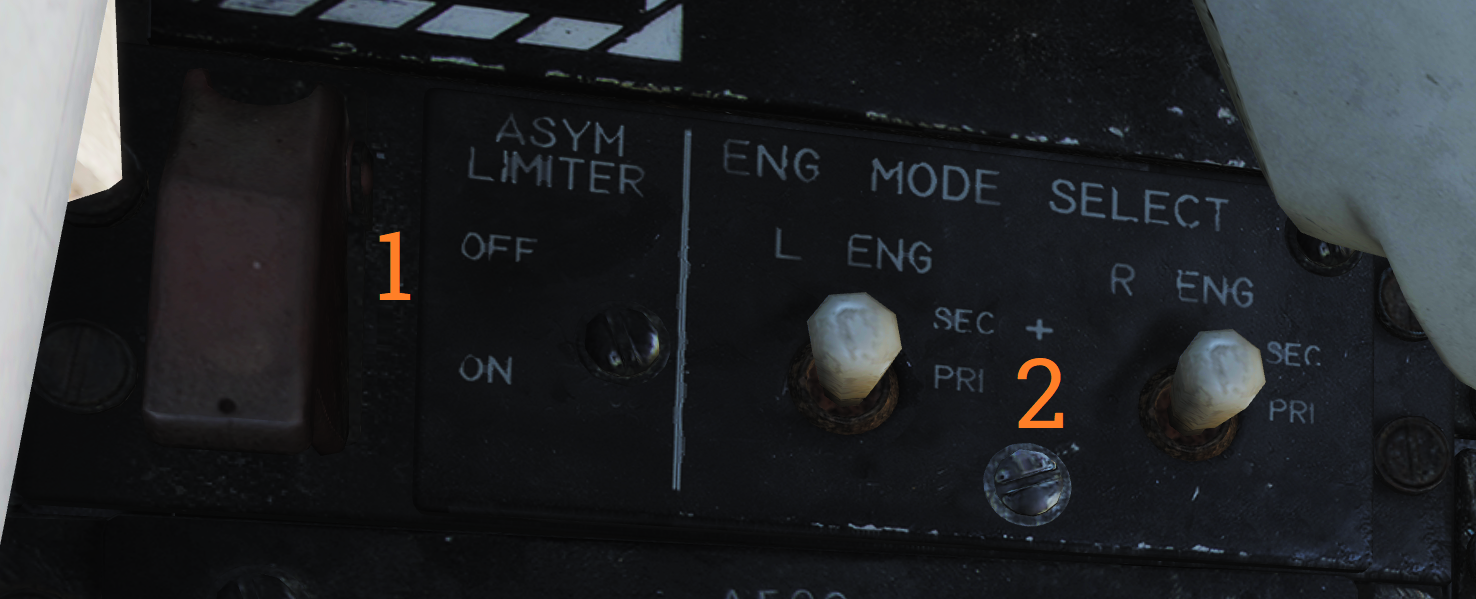
\includegraphics[width=0.6\textwidth]{asym1.png}
% \end{figure}
% ASYM LIMITER ( 1 )开关位于不对称推力限制器 / 发动机模式选择面板中,ASYM LIMITER 开关用来启用或禁用不对称加力推力限制器。开关默认位置为 ON 档位,保护盖关闭时将开关固定在 ON 档位。

% 同一面板中的其他两个开关为 ENG MODE SELECT (发动机模式选择)开关(2),两个开关分别用来设置左发动机(L ENG)和右发动机(R ENG)为 PRI (主要)模式或者 SEC (次要)模式。

% \begin{figure}[htb]
% 	\centering
% 	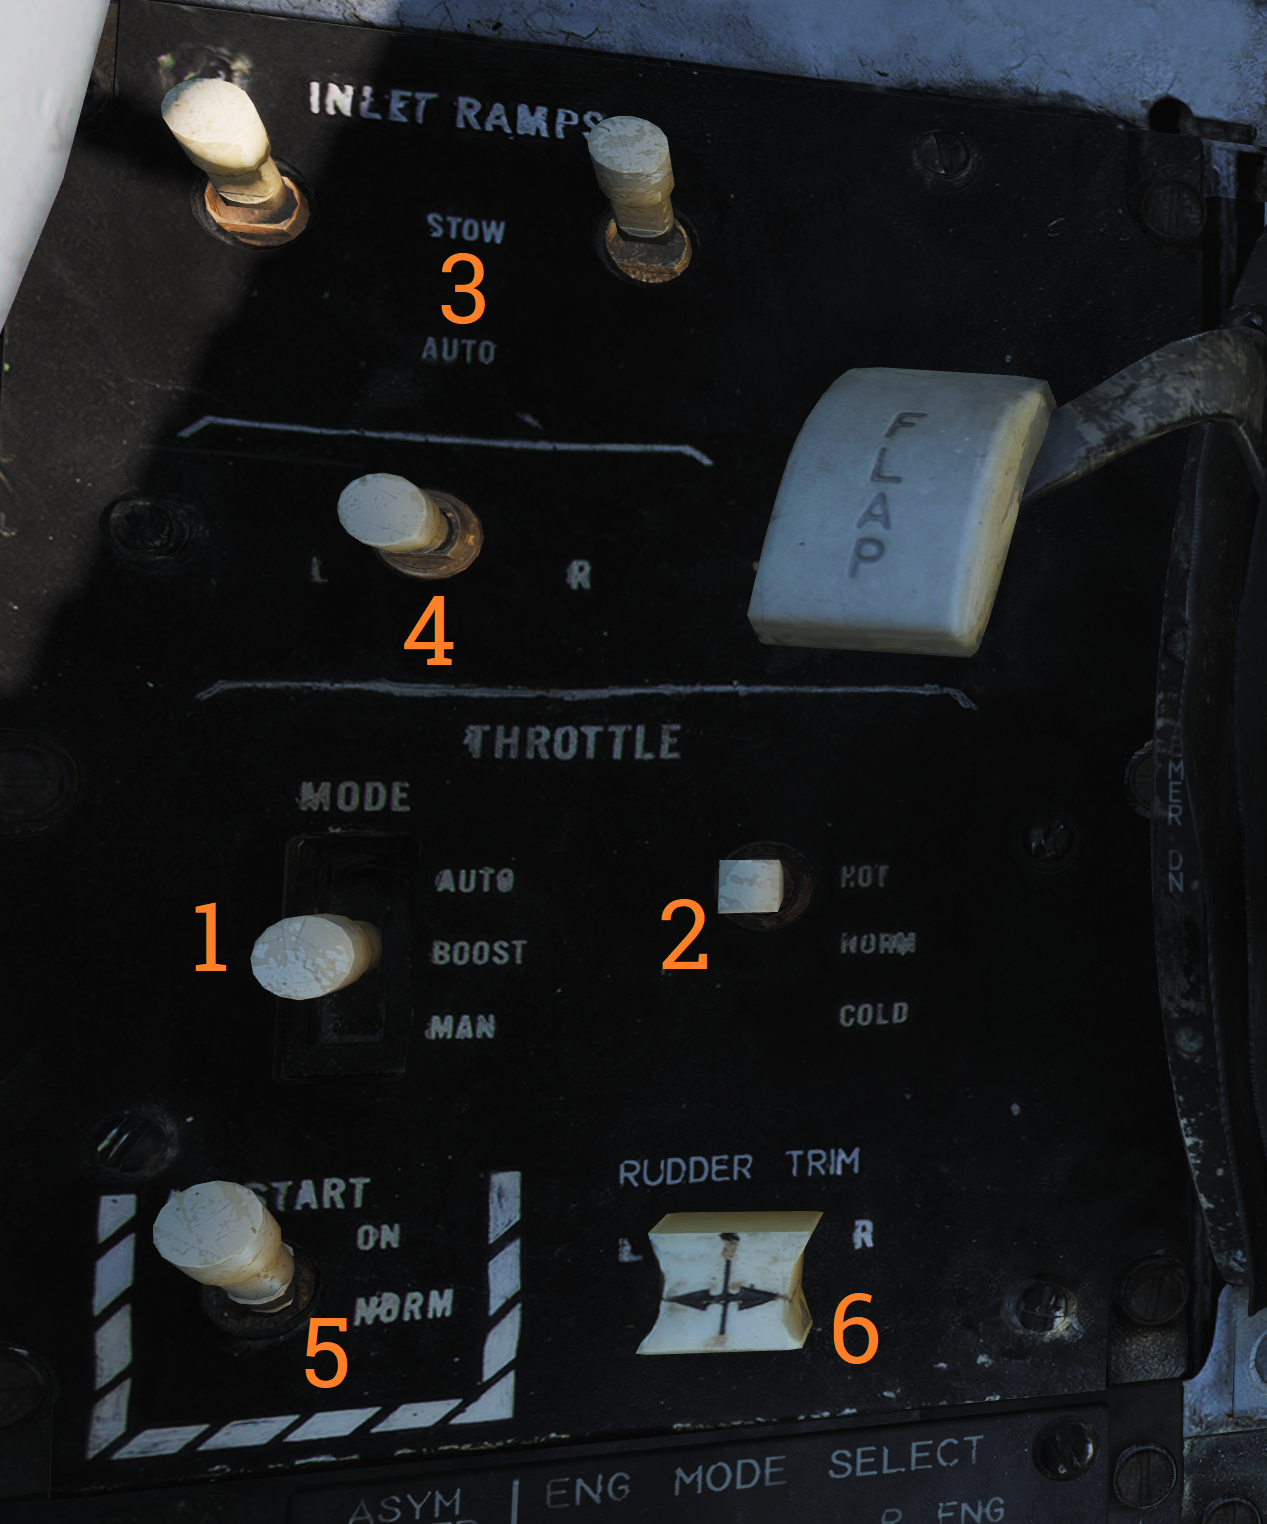
\includegraphics[width=0.6\textwidth]{inlet1.png}
% \end{figure}

% 进气道斜板 / 油门控制面板包含了大多数其它与发动机相关的控制开关。

% THROTTLE MODE (1)开关分别用来将油门模式设置为 AUTO 、 BOOST 或 MAN 模式,开关由弹簧归中至 BOOST 助力模式,如上所述,开关可由螺线管固定在 AUTO 档位。

% THROTTLE TEMP 开关也如上所述,用来控制自动油门系统的增益。

% INLET RAMPS ( 3 )开关用来启用( AUTO )或禁用,也就是收上( STOW )可调进气道斜板。

% 发动机起动开关(4)用于起动发动机至 20\% rpm,转速到达 20\% rpm 后可通过将对应的油门握把从 cut-off(关断)移动至 idle(慢车位)来起动发动机。如果飞机连接了外部气源,那么发动机则使用外部气源提供的空气来起动,如果没有连接外部气源则使用另一侧发动机提供的空气。当发动机转速到达 50\% rpm 时,起动开关将自动回到关闭/归中档位。如果起动开关在转速到达 50\% rpm 时没有自动归中,那么必须手动将其设置为归中(关闭)档位来防止损坏空气涡轮起动机。

% BACK UP IGNITION ( 5 )开关用来在主点火回路失效的情况下启用备用点火系统,通常通过将油门握把移动出 cut-off 档位来启用点火系统。

% \begin{figure}[htb]
% 	\centering
% 	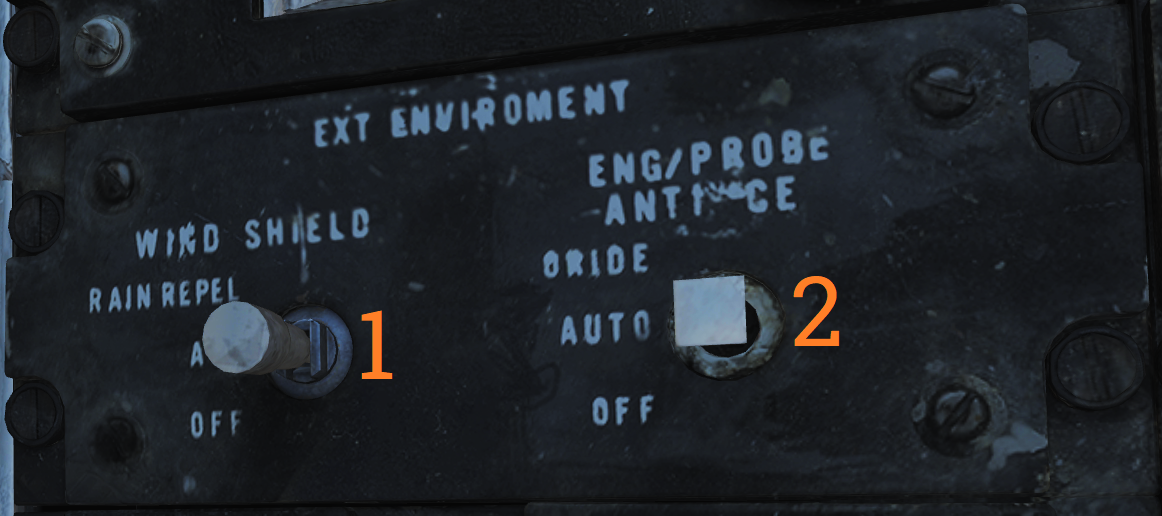
\includegraphics[width=0.6\textwidth]{externalenvironment1.png}
% \end{figure}
% 外部环境控制面板上的 ENG/PROBE ANTI-ICE (2)开关除了启用各个皮托管加热外,同时还启用发动机除冰以及进气道斜板除冰。开关拨至 ORIDE 将启用系统,开关拨动至 AUTO 档位时,如果探测到结冰,系统将被启用,开关拨至 OFF 档位将禁用系统。

% \subsection{发动机仪表组(EIG)及相关指示器和注意灯}
% \begin{figure}[htb]
% 	\centering
% 	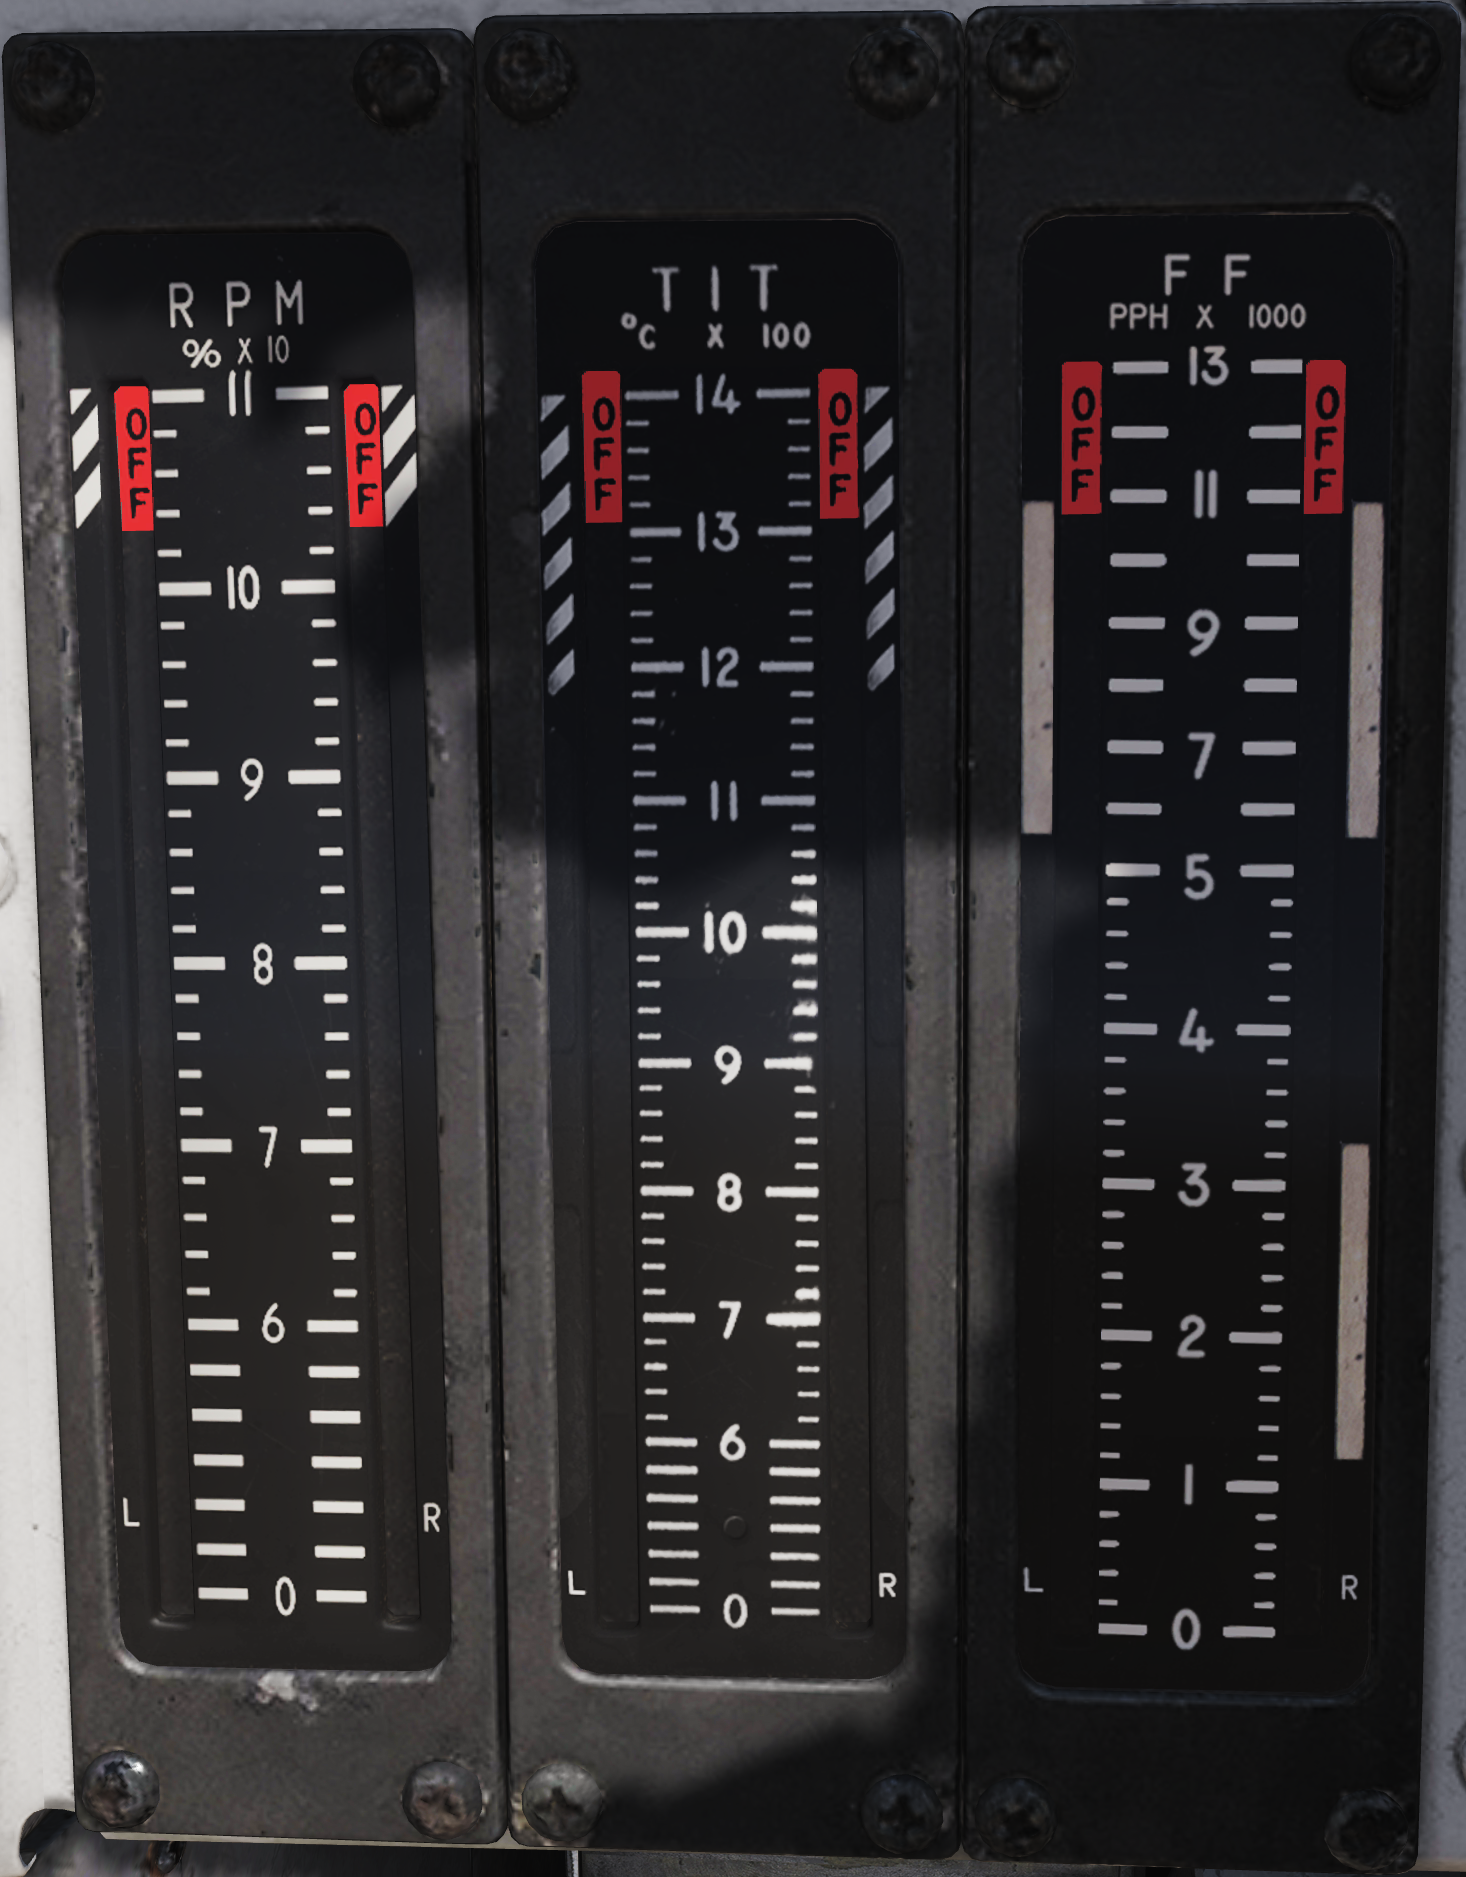
\includegraphics[width=0.6\textwidth]{instrument-group1.png}
% \end{figure}
% ENGINE INSTRUMENT GROUP (发动机仪表组)向飞行员显示 RPM (发动机转速)、 EGT (排气温度)以及 FF (燃油流量)以便监视发动机运转状态。

% 注意:上图中显示的是 TF30 发动机仪表组,而 F110 发动机仪表组将在不久后实装。

% \begin{figure}[htb]
% 	\centering
% 	
\includegraphics[width=0.6\textwidth]{exhaust1.png}
% \end{figure}
% 发动机喷口位置表显示相应发动机喷口当前的位置:0 表示喷口完全闭合,指针顺时针转动到最大值表示喷口完全张开。

% \begin{figure}[htb]
% 	\centering
% 	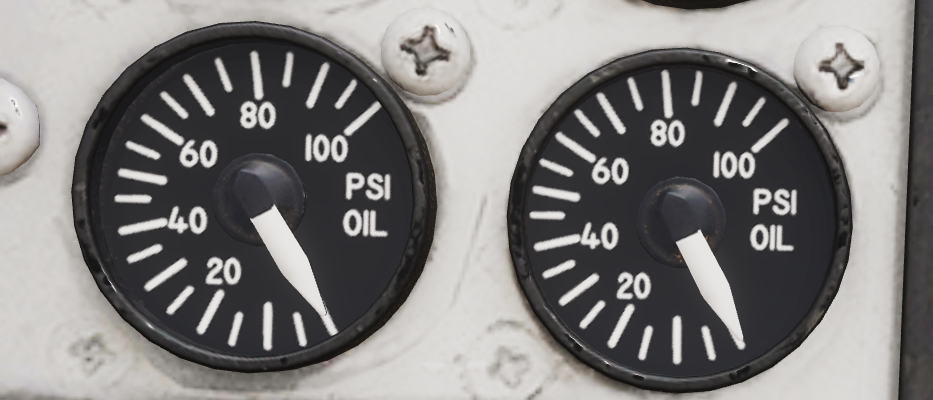
\includegraphics[width=0.6\textwidth]{oil1.png}
% \end{figure}
% 油压表中显示相应发动机中的滑油压力从而允许飞行员能够检查发动机中的滑油压力是否在正常水平。

% 与发动机运转相关的注意灯位于飞行员驾驶舱中,注意 - 提示灯面板中以及 HUD 两侧。

% 位于 HUD 两侧的提示灯为发动机失速报警灯,当检测到发动机失速时,报警灯将以 3Hz 的速率闪烁。HUD 左侧的报警灯用于指示左发压气机失速,右侧的报警灯则指示右发压气机失速。报警灯亮起的同时还将伴随调制出的 320Hz 的单音警告音。

% 左发压气机失速报警灯下方的指示灯中,其中一个指示灯为 AUTO THROT (自动油门)注意灯,当自动油门系统通过除使用油门模式开关以外的方法断开时,注意灯将会亮起10秒钟。

% 注意,提示灯面板中,发动机相关的注意灯和报警灯分别为:
% \begin{itemize}
% 	\item INLET ICE:注意灯亮起表示结冰信号器探测到结冰。
% 	\item L INLET 和 R INLET:注意灯亮起表示对应可调进气道系统的 AICS 系统出现了故障。
% 	\item OIL PRESS:注意灯亮起表示一侧发动机中的滑油压力过低。
% 	\item BLEED DUCT:注意灯亮起表示一侧发动机中出现高温空气泄漏。
% 	\item L RAMPS 和 R RAMPS:注意灯亮起表示对应的发动机进气道斜板没有锁定在指定的位置。
% 	\item START VALVE:注意灯亮起表示发动机起动机阀门开启。如果发动机起动后指示灯仍亮起,拨动发动机起动开关至归中位置。
% 	\item L ENG SEC 和 R ENG SEC:注意灯亮起表示其对应的发动机正在次要模式下运转。
% 	\item L GEN 和 R GEN:注意灯亮起表示其对应发动机的发电机不工作。
% 	\item L OIL HOT 和 R OIL HOT:注意灯亮起表示其对应的发动机中的滑油过热。
% 	\item L FUEL PRESS 和 R FUEL PRESS:注意灯亮起表示其对应发动机中,燃油泵的出口油压低于9 psi。
% 	\item RATS:注意灯亮起表示 RATS(航降减推系统)已启用。
% \end{itemize}

% \section{燃油系统}
% \begin{figure}[htb]
% 	\centering
% 	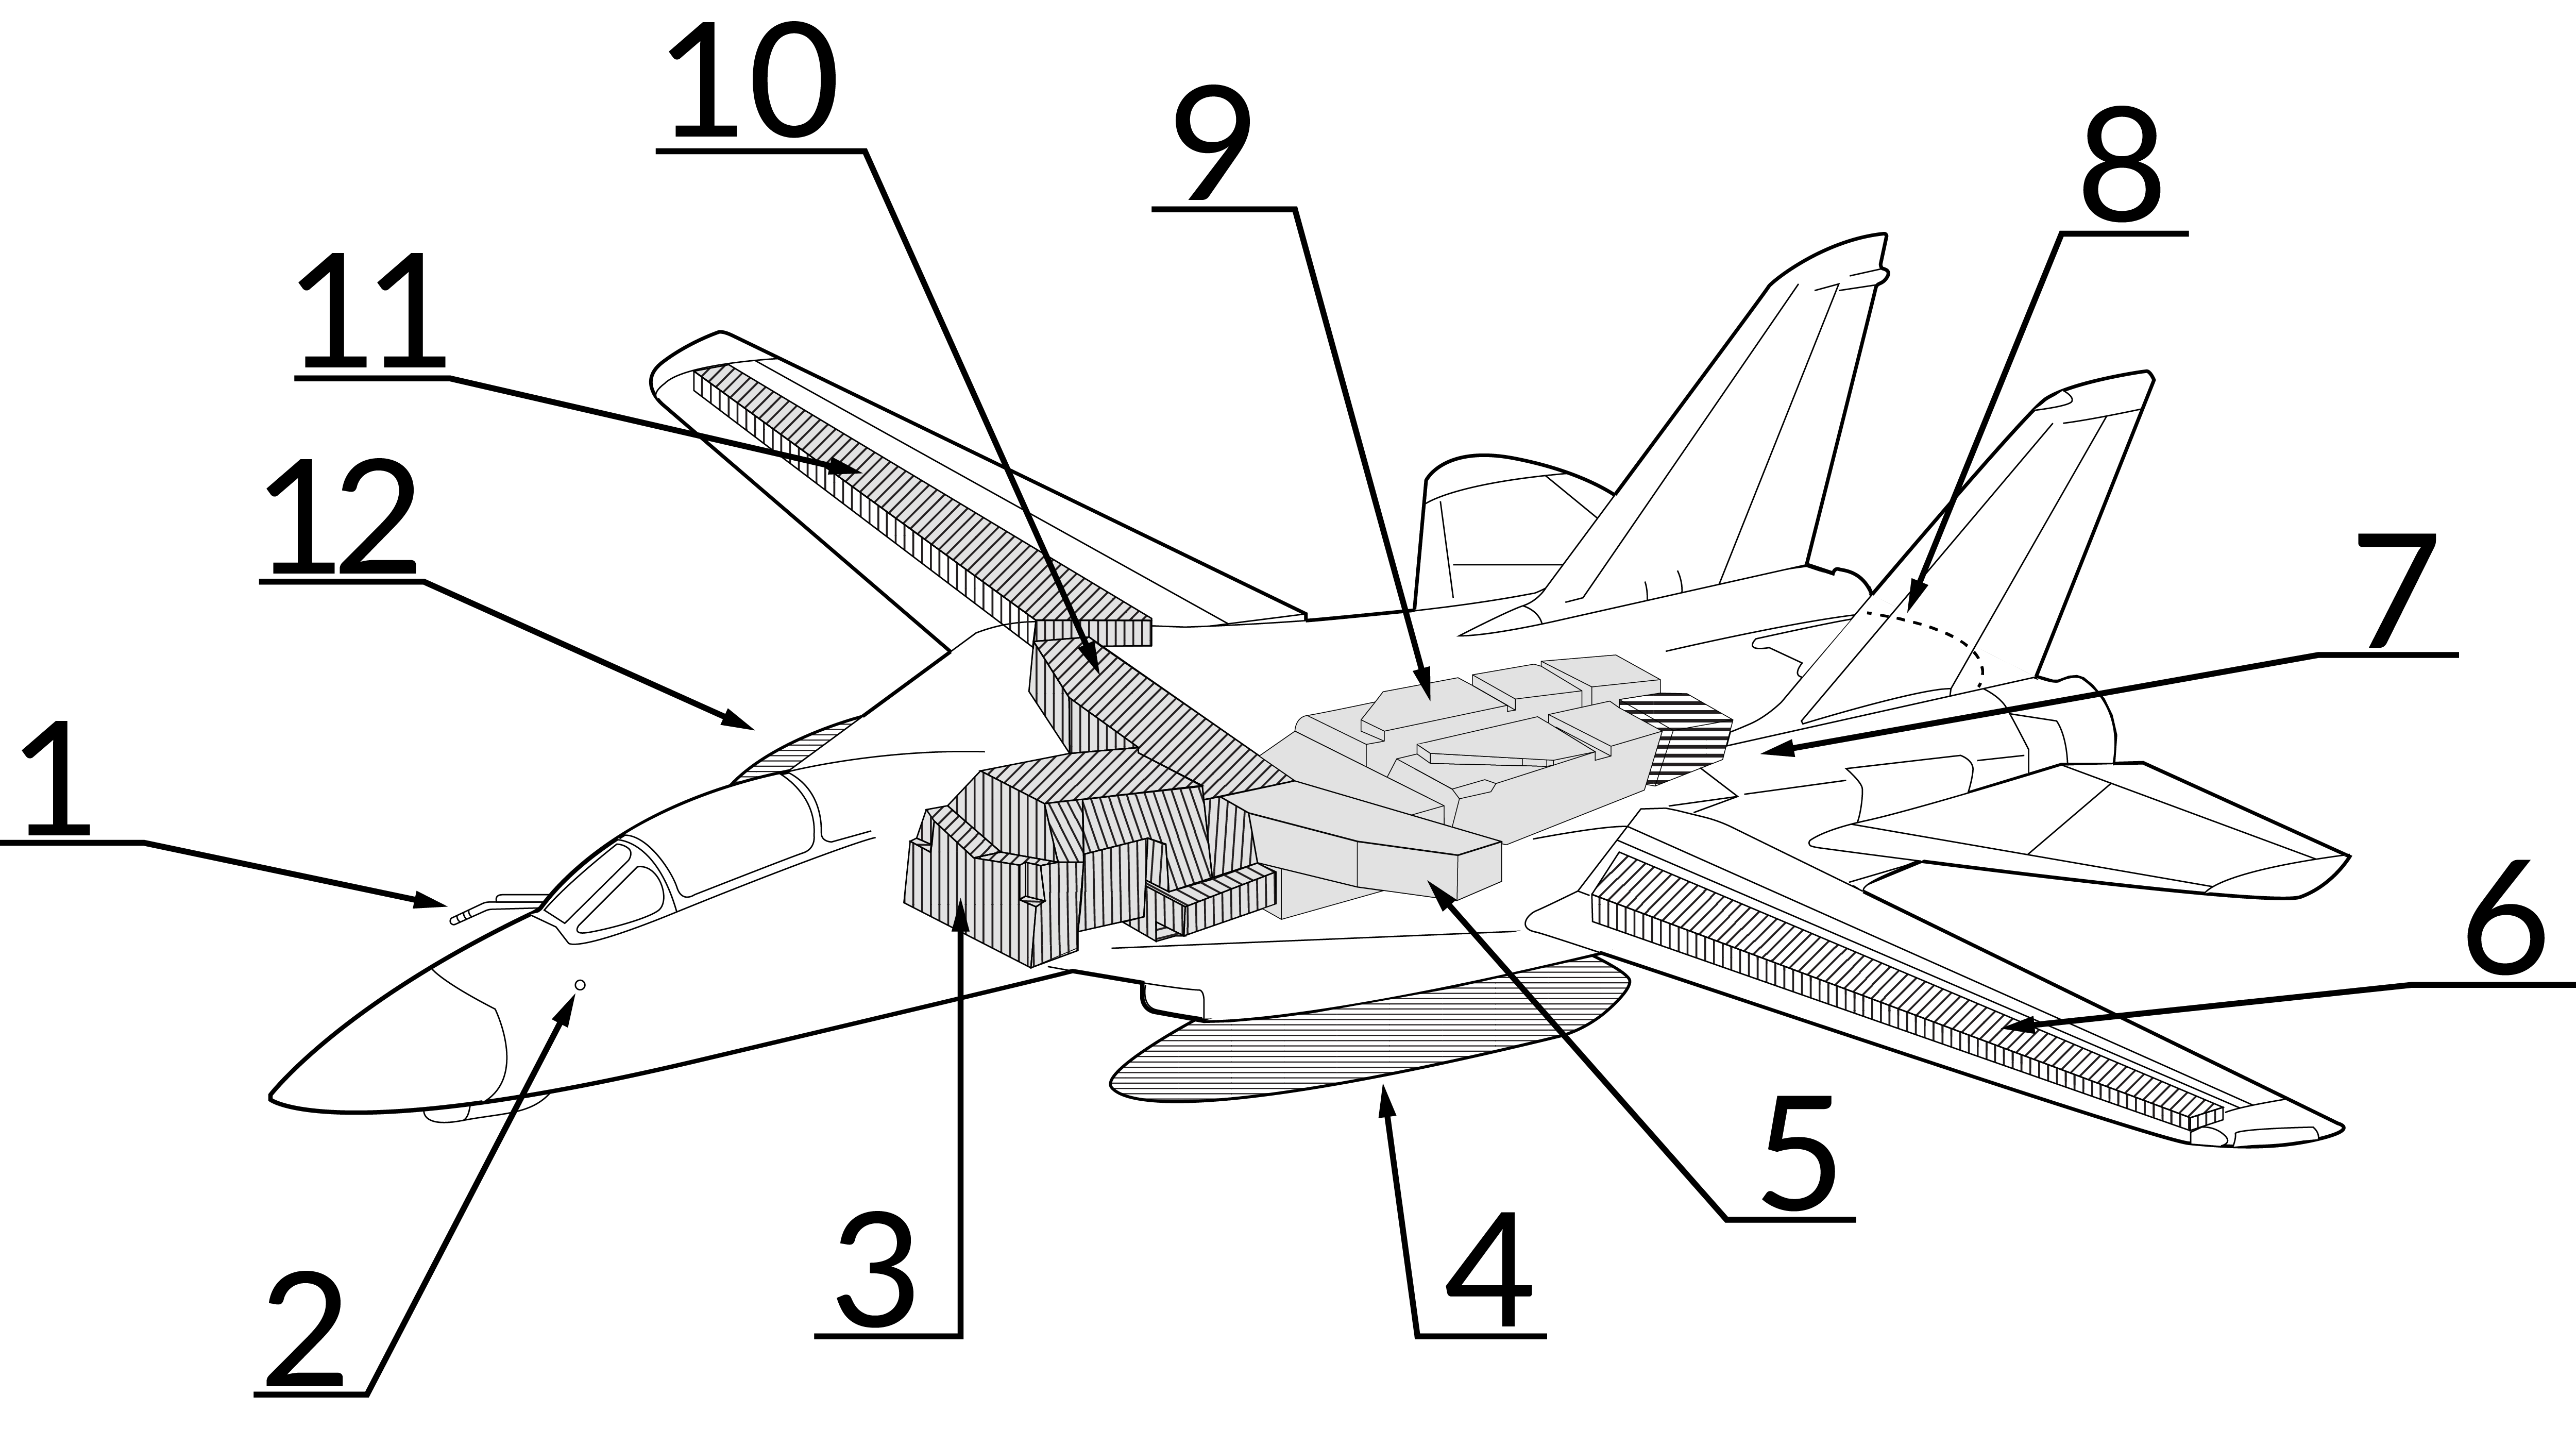
\includegraphics[width=0.6\textwidth]{tanks.png}
% \end{figure}

% 1 - 受油管,2 - 地面受油口(右侧),3 - 前机身油箱,4 - 左副油箱,5 - 左盒形梁油箱,6 - 左翼油箱,7 - 通气油箱,8 - 放油装置,9 - 后机身油箱,10 - 右盒形梁油箱,11 - 右机翼油箱,12 - 右副油箱。

% F-14 中主要用于储存燃油的为两个燃油供给系统,每台发动机各一个燃油供给系统。右发动机燃油供给系统由右机翼油箱、右盒形梁油箱和前机身油箱组成,而左发动机燃油供给系统由左翼油箱、左盒形梁油箱以及后机身副油箱。所以在进行油量表读数时,务必记住这一点。

% 如下表所示,飞机的可用燃油总量约为 20000 磅。

% \begin{table}[htb]
% 	\centering
% 	\begin{minipage}[t]{0.8\textwidth}
% 		\begin{tabularx}{\linewidth}{|l|X|X|X|X|}
% 			\hline
% 			油箱分组     & 磅    \\
% 			\hline
% 			前机身油箱   & 4,700 \\
% 			\hline
% 			后机身油箱   & 4,400 \\
% 			\hline
% 			右供油油箱组 & 1,600 \\
% 			\hline
% 			左供油油箱组 & 1,500 \\
% 			\hline
% 			机翼油箱     & 4,000 \\
% 			\hline
% 			副油箱       & 3,600 \\
% 			\hline
% 		\end{tabularx}
% 	\end{minipage}
% \end{table}

% \subsection{燃油量指示器和控制}
% \begin{figure}[htb]
% 	\centering
% 	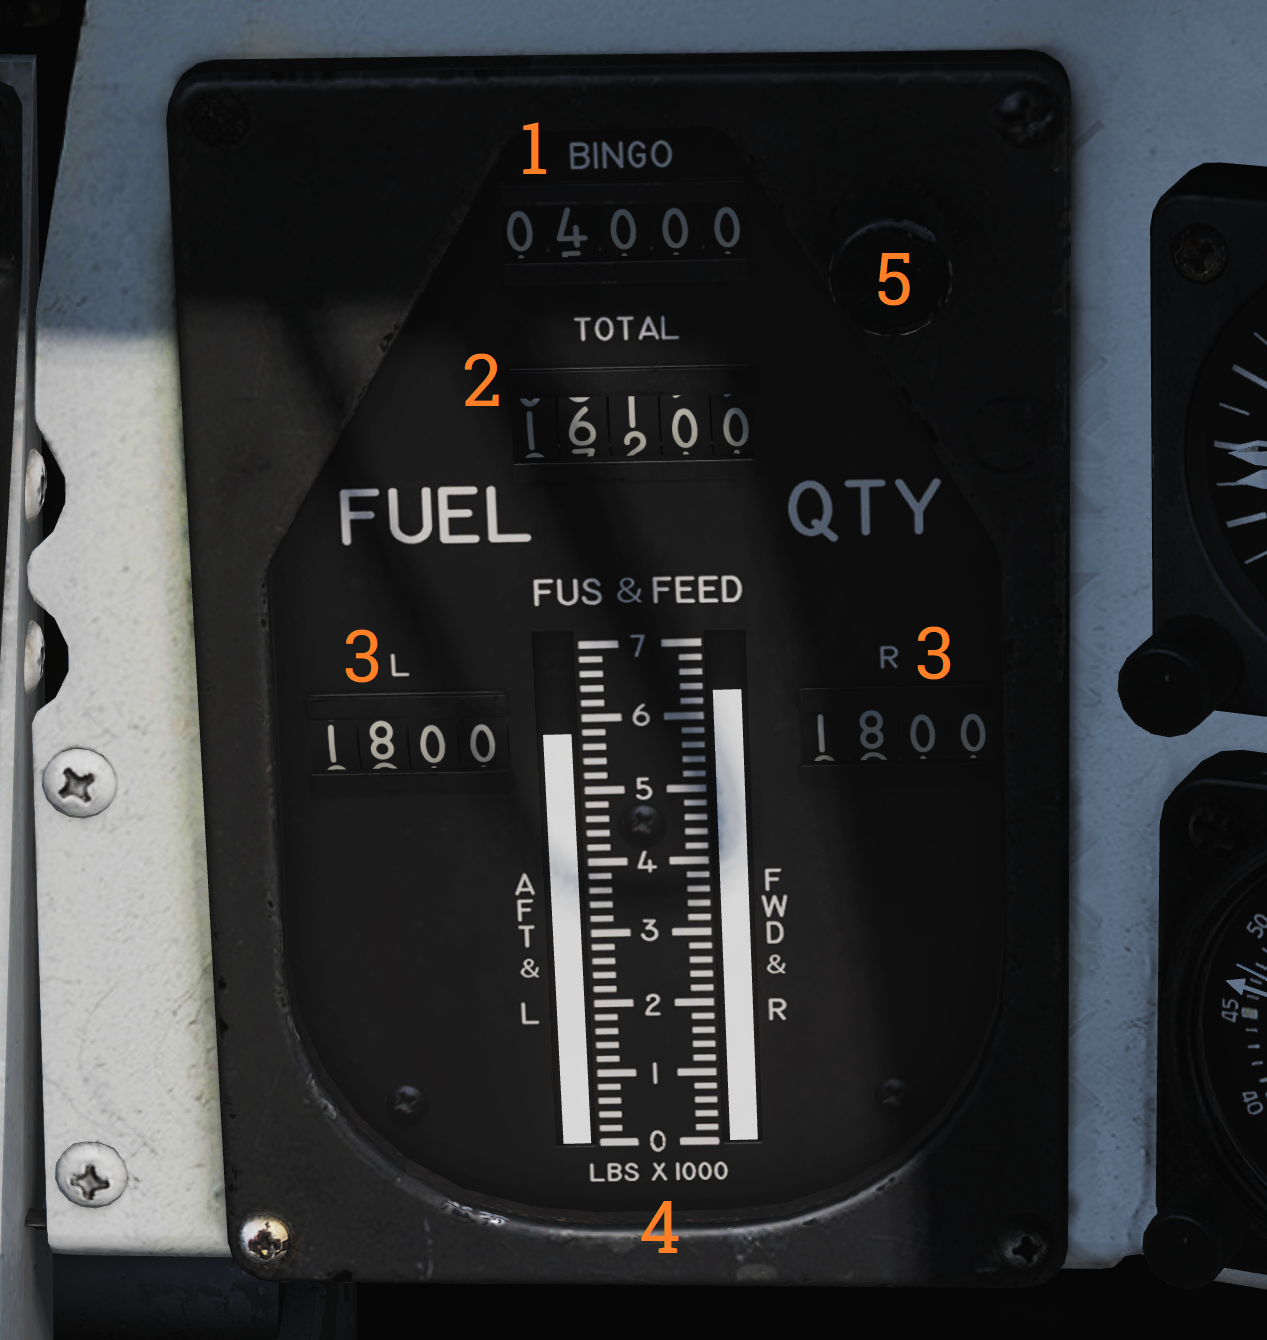
\includegraphics[width=0.6\textwidth]{fuelquantity1.png}
% \end{figure}
% 位于飞行员驾驶舱中右膝仪表板上的燃油量指示器用于指示飞机内部油箱和副油箱中的燃油量。

% 燃油量指示器中,最上方的指示器( 1 )显示当前设置的 BINGO (反航)油量,通过转动指示器旁边的旋钮( 5 )来设定所需的值。当剩余的燃油总量低于指示器中设定的值时,BINGO 注意灯就会亮起。

% TOTAL (2)指示器显示飞机所有油箱中的燃油总量。

% 一般情况下, L 和 R ( 3 )分别显示左/右供油油箱组的燃油量。燃油管理面板中的摇臂开关用于选择显示机翼油箱(WING)或副油箱(EXT)的燃油量,但摇臂开关由弹簧归中显示供油油箱组(FEED)的燃油量。当指示器显示机翼油箱或副油箱油量时,L(左侧)计数器将指示左翼油箱或左侧副油箱中的燃油量,R(右侧)计数器则指示右翼油箱或右侧副油箱的燃油量。

% FUS \& FEED 条状指示器(机身油箱和供油油箱组)以千磅为单位显示 AFT \& L (后机身油箱和左供油油箱组)以及 FWD \& R (前机身油箱和右供油油箱组)的燃油量。

% 另外,RIO 驾驶舱中也含有一个燃油量指示器,指示器位于右仪表板中。这个指示器只能显示所有油箱的燃油总量(详见 燃油总量表)。

% \begin{figure}[htb]
% 	\centering
% 	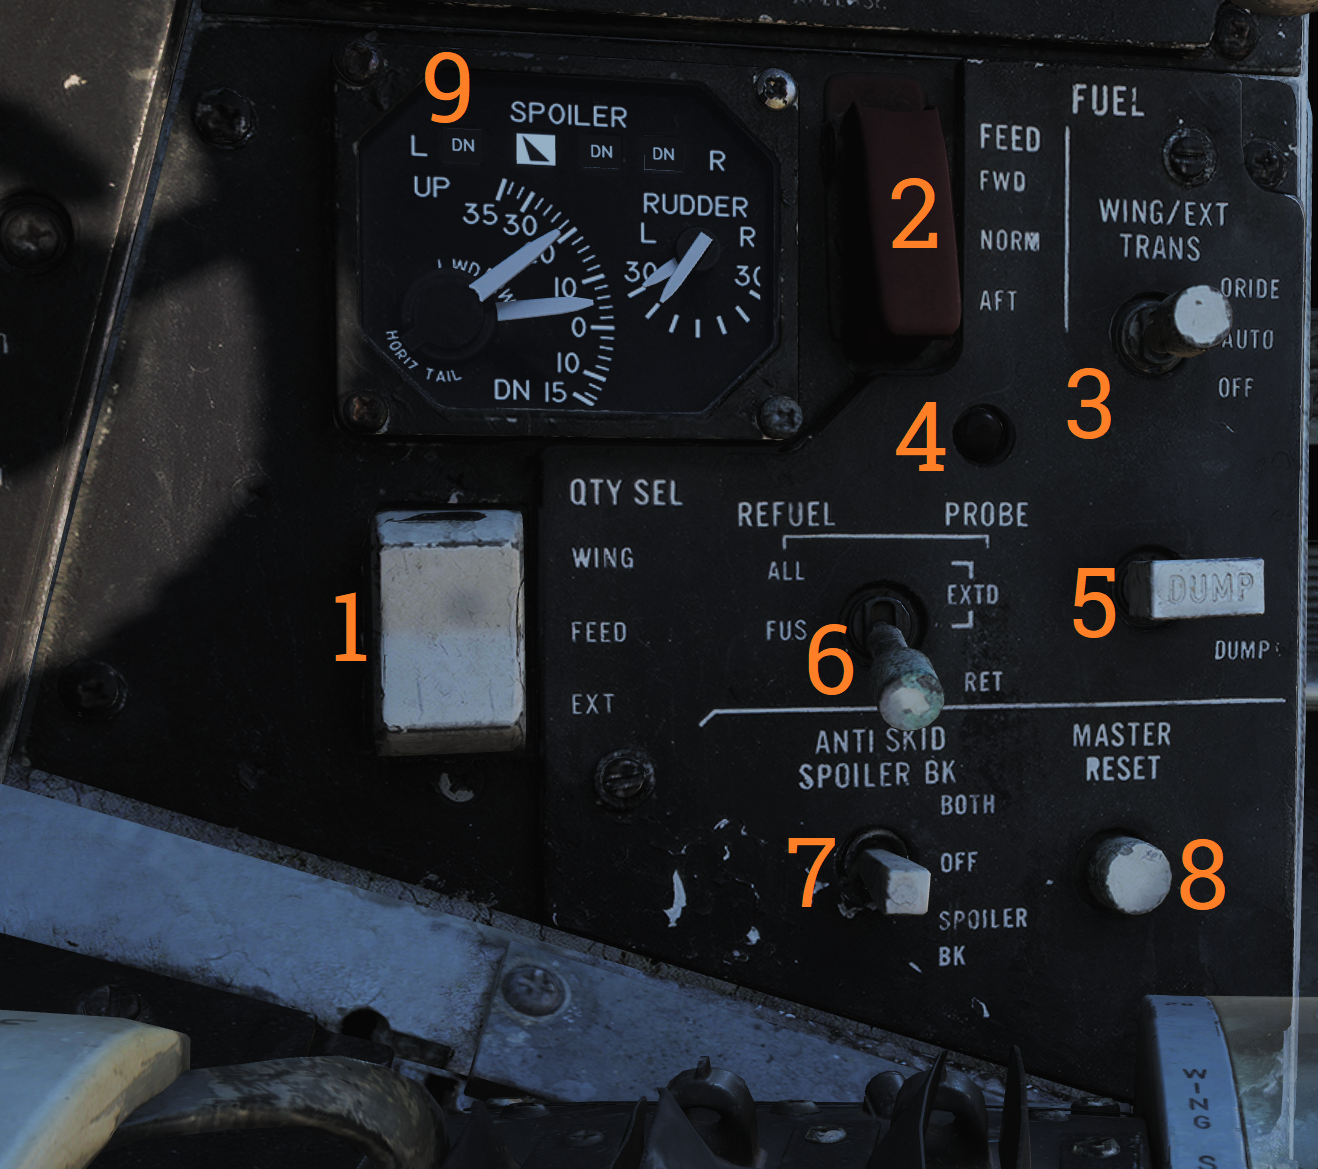
\includegraphics[width=0.6\textwidth]{fuel2.png}
% \end{figure}

% 位于飞行员驾驶舱中左侧垂直控制台上包含有适用于燃油系统的控制开关和按钮。

% QTY SEL (1)摇臂开关在上文关于 L \& R 燃油量指示带的介绍中有详细说明。

% 飞行员可以使用 FEED 开关来通过选择 FWD 档位(前机身油箱和剩余右发供油所使用的油箱)或 AFT 档位(后机身油箱和剩余左发供油所使用的油箱)修正由于单发停车或燃油供给管路故障所导致两侧油箱燃油量不平衡,而不像 NORM 档位中左/右发动机燃油供给分别向对应的发动机输送燃油。当保护盖关闭时,这个开关会被锁定在 NORM 档位。

% WING/EXT TRANS 开关用来控制机翼到发动机供油系统以及副油箱到发动机供油系统的燃油传输。一般情况下使用的 AUTO 档位将在起落架收上后立刻启用机翼/副油箱燃油传输。开关拨动至 ORIDE 档位时,无论起落架当前的位置,机翼/副油箱的燃油传输都将被启用,绕过起落架收上检测从而允许当飞机处于地面或在输油系统中发生电气故障时启用机翼/副油箱燃油传输。此外,开关位于 OFF 将禁用机翼/副油箱传输,但是当在 MTS(主测试)面板中选择 INST 档位进行测试、受油管设置为 ALL EXTD 或放油时,开关将被自动超控至 AUTO 档位。

% 使用 DUMP (5)开关可以通过河狸尾巴放油装置来将燃油放出,同时开关还会启用所有输油系统,使得除了机身油箱外,还能将机翼和副油箱中的燃油放出。如果机轮负重或者减速板未完全收起,那么放油将被禁止。

% 注意:尽管从技术上来说,放油过程中是可以开启加力燃烧室的,但是这样有可能会点燃放出的燃油,因此禁止在放油时进行加力燃烧。

% \subsection{空中受油}
% 上文所讲的燃油管理面板还可以对空中受油系统进行控制。

% REFUEL PROBE (6)开关用于控制受油管伸出以及设置燃油系统来进行接收。两个伸出档位(EXTD)分别为 ALL 档位——启用所有油箱受油,包括机翼油箱和副油箱, FUS 档位——启用仅机身油箱受油。开关位于 ALL 档位时,机翼和副油箱的输油将被禁用从而使所有油箱受油。开关位于 RET (收起)档位时,受油管收回并恢复一般燃油系统运作。

% 注意:开关拨至 EXTD ALL 将复位 WING/EXT TRANS 开关至 AUTO 档位。

\section{失火探测和灭火系统}

\subsection{失火探测系统}
F-14 的失火探测系统含有两个火焰感测回路,每台发动机各一个。

如果整个回路中每一处都探测到温度都超过 600°F(约 316°C),或在任意 6 英寸范围内探测到温度超过 1,000°F(约 538°C)便会触发失火探测回路。触发左探测回路使 ACM 面板中左发失火报警灯亮起,触发右探测回路使右发起火报警灯亮起,详情 空战格斗面板 。

此外,F-14 中还有多个设计用于探测发动机内热空气泄露的传感器,如果探测空气温度高于575 °F (约302 °C),飞行员驾驶舱中 注意 - 提示灯面板 上的 BLEED DUCT 注意灯将亮起。

\subsection{灭火系统}

\begin{figure}[h]
	\centering
	\begin{subfigure}{0.45\textwidth}
		\centering
		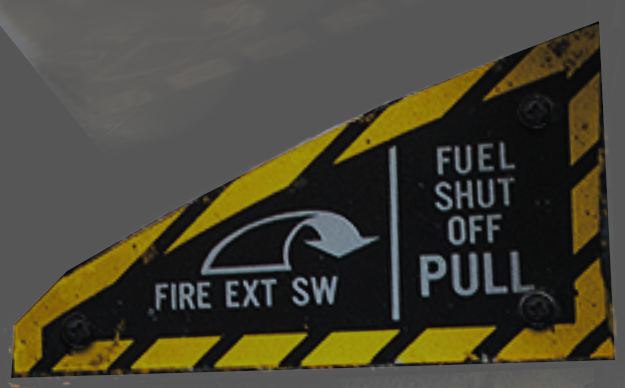
\includegraphics[width=1.0\textwidth]{left1.png}
	\end{subfigure}
	\hspace{1em}
	\begin{subfigure}{0.45\textwidth}
		\centering
		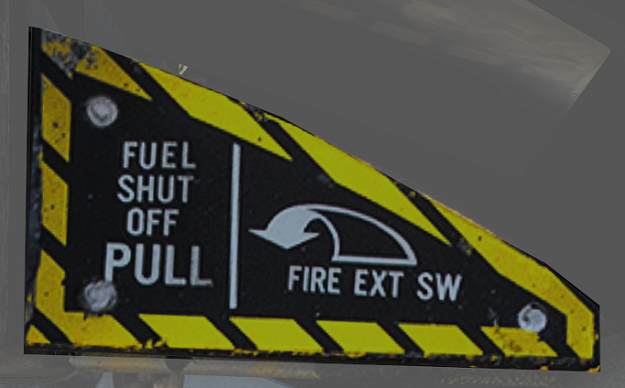
\includegraphics[width=1.0\textwidth]{right1.png}
	\end{subfigure}
\end{figure}

F-14 的灭火系统包含两个装有灭火剂的灭火瓶,灭火剂可以被注入飞行员选择的发动机中。虽然系统包含两瓶灭火瓶,但是两瓶灭火瓶会同时注入灭火剂使得灭火系统成为一次性系统,一次只能扑灭一台发动机中的火灾。

由于灭火剂的有效性取决于在火被熄灭前留在发动机内的时长,因此,在飞机空速较低的情况下,灭火剂的灭火效果更佳,这是因为在低速下,需要更长的时间来将灭火剂从发动机中吹出。灭火剂毒性低,旨在有效灭火的前提下尽可能减少对发动机造成的损伤。

飞行员可以抽出失火发动机相应的 FUEL SHUT OFF 手柄(见上图),并按下该手柄后面的灭火器按钮来激活灭火系统。拉起手柄将切断对应发动机的燃油供给,而灭火器按钮则将释放灭火剂注入到发动机中。

还有两个提示灯连接到灭火系统中,每个提示灯用来指示其中一个灭火瓶中的压力较低。 ENG FIRE EXT 表示主灭火瓶中压力较低, AUX FIRE EXT 表示辅助灭火瓶中压力较低。两个提示灯都位于飞行员驾驶舱中注意-提示面板上,详见 注意 - 提示灯面板 。

成功启用灭火系统后系统的两个提示灯将会亮起,并且还将指示是否错误释放瓶中的压力。

\subsection{失火探测和灭火系统测试}
这两个系统都可以通过选择位于主测试面板中的 FIRE DET/EXT 档位来进行测试(详见 主测试面板 )。测试中,如果各自的回路正常工作,那么 ACM 面板中的两个失火报警灯将会亮起;如果测试中灭火系统正常工作,那么主测试面板中的 GO 指示灯将会亮起。如果在测试中,主测试面板中 NO GO 或没有指示灯亮起,那么表示灭火系统或测试电路存在问题。

% \section{电气系统}
F-14 中所有主要的电力都由两台发动机驱动的 AC(交流)发电机来提供。连接到发动机减速箱的每台发电机都能发出足够的电力来驱动飞机中所有的系统。

F-14 装备了两台整流变压器来作为 DC(直流)发电为系统提供 28V DC(直流电),同样每台整流变压器都可以单独驱动飞机中所有需要用到 DC 的设备。

F-14 在前轮后方包含有一个使用 AC 电源的外部电源插座,外部电源插座能够为飞机提供 AC 和 DC(通过整流变压器)。当一台内部发电机正常工作时,外部电源将自动从飞机电气系统中断开。

\subsection{应急电力}
F-14 中包含有一台由联合液压系统驱动的应急发电机,应急发电机可以发出有限的电力来提供 AC (交流电)和 DC(直流电)。如果系统失去由两台主发电机提供的电力,应急发电机将在1秒内接管关键飞行系统的供电。

\subsection{控制器和指示器}
\begin{figure}[htb]
	\centering
	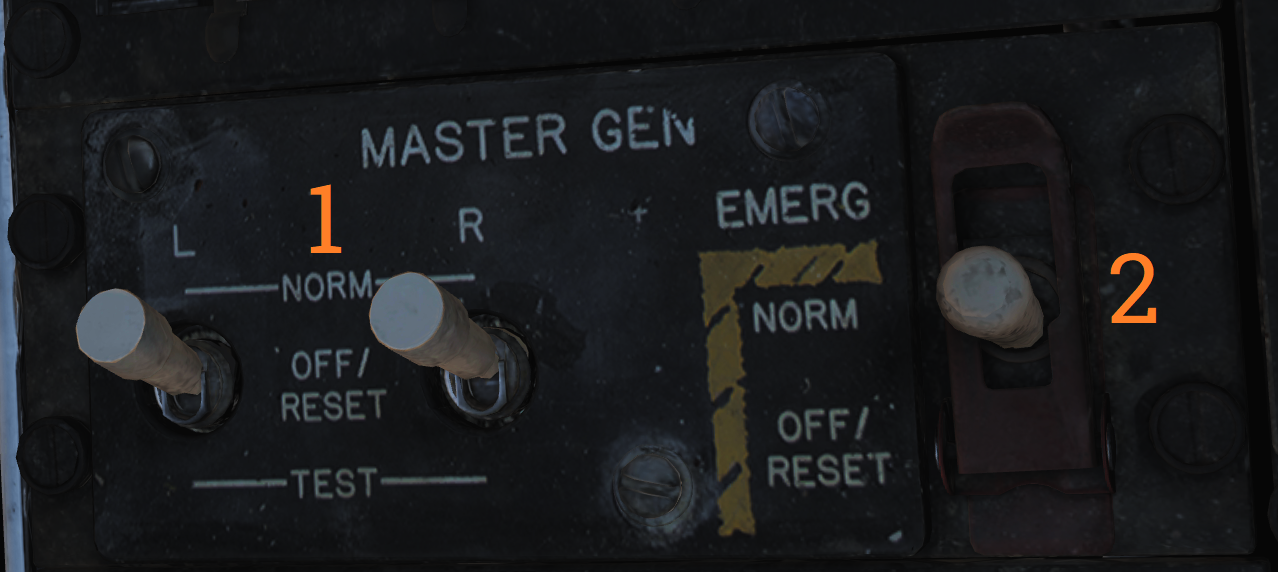
\includegraphics[width=0.6\textwidth]{generator1.png}
\end{figure}

电气系统的控制开关全部位于主发电机控制面板中。

MASTER GEN ( 1 )开关控制主发电机到电力总线的连接。 NORM 档位用于将对应一侧的发电机连接到总线。 OFF/RESET 档位用于断开发电机与总线的连接,并且复位任何由于供电超出正常限制而切断的保护电路。TEST 档位用于起动发电机,但不会将发电机连接到电力总线,从而在不影响其他飞机系统的情况下对发电机进行测试。开关被锁定在 NORM 档位,提起开关后才能将其拨回 OFF/RESET 档位。

EMERG ( 2 )开关用于控制应急发电机。开关位于 NORM 档位时,如果主发电机发生故障,应急发电机将自动连接到应急总线。OFF/RESET 档位将禁用应急发电机,同时还复位相关保护电路(如果发生跳闸)。此开关被保护盖固定在 NORM 档位,需要升起保护盖才能将开关拨至 OFF/RESET 档位。

电气系统相关的注意/提示灯位于飞行员驾驶舱 注意 - 提示灯面板 中。L GEN 和 R GEN 指示灯亮起表示对应的发电机没有正常工作。可能是由于发电机故障或驱动发电机的发动机没有运转。

TRANS/RECT 提示灯亮起表示一个或全部整流变压器没有正常工作。

应急发电机可以通过 主测试面板 中的 MASTER TEST 开关,选择 EMERG GEN 档位对发电机进行测试。GO 指示灯亮起表示测试完成。 发生故障时, NO GO 指示灯将会亮起。

\subsection{断路器}
F-14 的断路器位于飞行员的左/右膝仪表板以及 RIO 座椅后部的左侧和右侧。通过弹出断路器来从过电流中保护飞机的系统并隔离消耗太多电流的系统。断路器弹出时,断路器中将会出现一根白线表示已弹出。可以通过按下断路器来将断路器复位,也可以手动抽出断路器。

断路器实装至 DCS 时,我们会在此处详细描述各个断路器的功能。

% \section{液压系统}

% \section{机翼后掠系统}

% \section{飞行控制系统}

% \section{起落架系统}

% \section{弹射起飞和拦阻装置}

% \section{环境控制系统(ECS)}

% \section{供氧系统}

% \section{飞行仪表}

% \section{座舱盖}

% \section{弹射系统}

% \section{灯光系统}

% \section{抛离系统}

% \section{中央大气数据计算机(CADC)}

% \section{AN/AWG-9武器控制系统(WCS)}

% \section{AN/APX-76 IFF问询器}

% \section{电视摄像套件(TCS)}

% \section{LANTIRN}

% \section{AN/ALR-67雷达告警接收机(RWR)}

% \section{AN/ALE-39对抗弹射套件}

% \section{AN/ALQ-126 DECM}

% \section{导航}

% \section{通信系统}

